\section{Hyperparameter Tuning}
\label{sec:app:hyperparameter}
For both supervised fine-tuning and instruction tuning, we pre-set the effective batch size to 8, and tune the learning rate within \{$2\times 10^{-5}$, $2\times 10^{-6}$, $2\times 10^{-7}$\}.
Each model is fine-tuned for 3 epochs on the supervised fine-tuning tasks and 5 epochs on Tulu for instruction tuning.
In both settings, we adopt an AdamW optimizer with a linear learning rate scheduler.
The optimizer is warmed up for the first $3\%$ of the training time.

\section{Prediction Generation Method}
\label{app:pred_gen}
\begin{table}[t]
\small
\centering
\begin{tabular}{@{}llrrr@{}}
\toprule
\textbf{Dataset}       & \textbf{Model} & \multicolumn{1}{l}{\textbf{Free}} & \multicolumn{1}{l}{\textbf{Constrained}} & \multicolumn{1}{l}{\textbf{TokenProb}} \\ \midrule
\multirow{2}{*}{MNLI}  & Fine-tuned     & 0.786                                        & 0.791                                             & 0.792                                         \\
                       & BASE           & 0.0                                          & 0.0                                               & 0.327                                         \\ \arrayrulecolor{black!30}\midrule
\multirow{2}{*}{RTE}   & Fine-tuned     & 0.658                                        & 0.662                                             & 0.66                                          \\
                       & BASE           & 0.0                                          & 0.0                                               & 0.241                                         \\ \arrayrulecolor{black!30}\midrule
\multirow{2}{*}{Paws}  & Fine-tuned     & 0.871                                        & 0.878                                             & 0.878                                         \\
                       & BASE           & 0.0                                          & 0.0                                               & 0.558                                         \\ \arrayrulecolor{black!30}\midrule
\multirow{2}{*}{STS-B} & Fine-tuned     & 0.775                                        & 0.741                                             & 0.744                                         \\
                       & BASE           & 0.0                                          & 0.0                                               & 0.964                                         \\ \arrayrulecolor{black}\bottomrule
\end{tabular}
\caption{Performance of final checkpoint with different prediction generation method.}
\label{app:tab:pred_gen_method}
\end{table}
For classification tasks, we examine three different prediction generation methods: Free Generation (\texttt{Free}), Constrained Generation (\texttt{Constrained}), and Token Probability (\texttt{TokenProb}), the results are shown in Table~\ref{app:tab:pred_gen_method}.
In \texttt{Constrained}, we force the output to include at least one label in the acceptable label set.
In \texttt{TokenProb}, we compare the logits of acceptable labels, and select the label with the highest score as final output.
This ablation study is conducted only on the BASE and fine-tuned versions of final checkpoint of the pre-trained model.
We find that, although prediction generation methods bring less effect to the evaluation result of a fine-tuned model, BASE variants suffer much more from not knowing the desired output.
Therefore, we proceed all the classification experiments with \texttt{TokenProb}.

\subsection{Label and Tokenizations}
Depending on the tokenizer variant, the label text may be tokenized differently, leading to evaluation unreliability.
For example, in paraphrase detection, the model could assign probability on both ``\texttt{yes}" and ``\texttt{ yes}" (the same label with a prefix space).
This behavior is reported and explored in various related work \cite{sun-etal-2023-tokenization, batsuren2024evaluating, singh2024tokenization}.
In this study, we leniently regard all individual tokens that contains the whole label or part of the label along with some special charcters that do not affect the semantic as an acceptable target label.


\section{Task Format}
We adopt the task format from \cite{yang2024unveiling}, with an additional task format of input-output.
How each dataset is formated can be found in Table~\ref{tab:app:promptformat}.

\section{GPU Hours per-Experiment}
\label{sec:app:gpuhours}
We show a table of GPU hours spent for each experiment in Table~\ref{app:tab:GPU-hours}.
The total number of GPU hours spent in this project is approximately 1067 A100 hours. We lose track of the GPU hours spent on preliminary experiments, so a lower-bound estimation is reported.
\begin{table*}[t]
\centering
\begin{tabular}{@{}crrrr@{}}
\toprule
\multicolumn{5}{c}{\textbf{Prelinminary Experiments}} \\ \midrule
\multicolumn{3}{l}{\textbf{Description}} & \multicolumn{2}{l}{\textbf{GPU Hours}} \\ \arrayrulecolor{black!30}\midrule
\multicolumn{3}{l}{Instruction Tuning on LIMA, TULU, and NaturalInstructions} & \multicolumn{2}{r}{$\sim$300} \\
\multicolumn{3}{l}{Model Performance Verification, Dataset Selection} & \multicolumn{2}{r}{120} \\ \arrayrulecolor{black}\midrule
\multicolumn{5}{c}{\textbf{Instruction Tuning}} \\ \arrayrulecolor{black}\midrule
\multicolumn{3}{l}{Instruction Tuning} & \multicolumn{2}{r}{360} \\
\multicolumn{3}{l}{Evaluation} & \multicolumn{2}{r}{10} \\
\multicolumn{3}{l}{Total} & \multicolumn{2}{r}{\textbf{370}} \\ \arrayrulecolor{black}\midrule
\multicolumn{5}{c}{\textbf{Fine-Tuning}} \\ \arrayrulecolor{black!30}\midrule
\multicolumn{1}{l}{} & \multicolumn{1}{l}{\textbf{XSum}} & \multicolumn{1}{r}{\textbf{SocialIQa}} & \multicolumn{1}{l}{\textbf{MNLI}} & \multicolumn{1}{l}{\textbf{Paws}} \\ \arrayrulecolor{black}\midrule
\textbf{Training} & 12 & 6 & 4.6 & 5.3 \\
\textbf{Evaluation} & 8 & 5.3 & 3 & 2 \\
\textbf{OOD Evaluation} & 96 & 32 & 11 & 25.6 \\
\textbf{CrossTask Evauation} & 5.2 & 6.5 & 7.7 & 8.15 \\
\textbf{Task Format Evaluation} & 16 & 12.8 & 6 & 4 \\
\textbf{Total} & \multicolumn{4}{c}{137.2 + 62.6 + 32.3 + 45 = 277.1} \\ \arrayrulecolor{black}\bottomrule
\end{tabular}
\caption{GPU hours for each experiment. The total amount of GPU hours spent in this project is approximately 1067 A100 hours.}
\label{app:tab:GPU-hours}
\end{table*}

\section{Per-dataset Figures}
\label{sec:app:per-ds-ckpt-figures}
\begin{figure*}[t!]
    \centering
    \begin{subfigure}[b]{0.3\textwidth}
    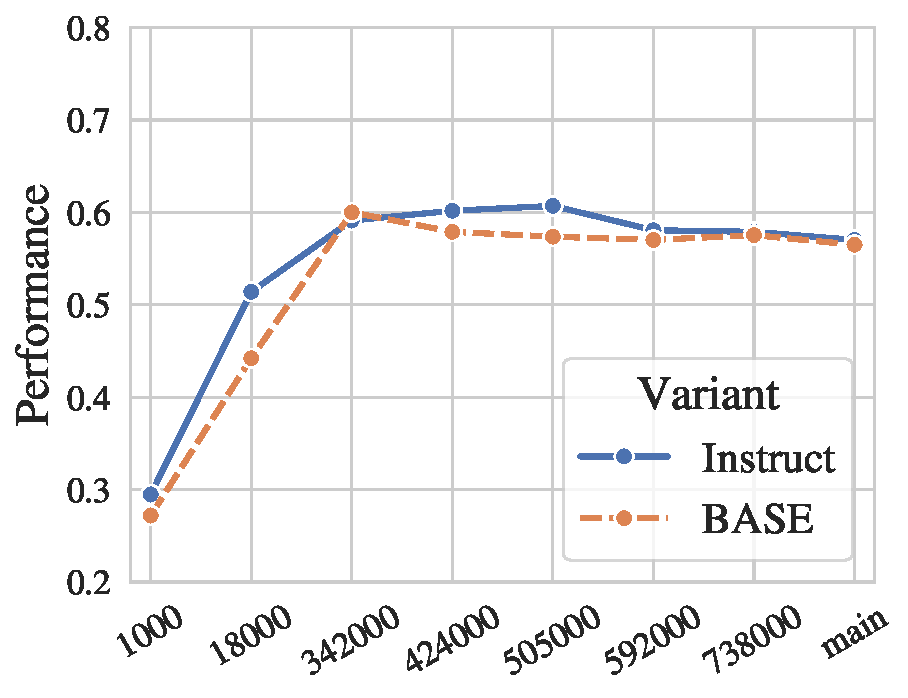
\includegraphics[width=\the\columnwidth]{figures/fig_files/it_ckpts/it_evalarc_easy.pdf}
        \caption{ARC Easy}
    \end{subfigure}%
    ~ 
    \begin{subfigure}[b]{0.3\textwidth}
    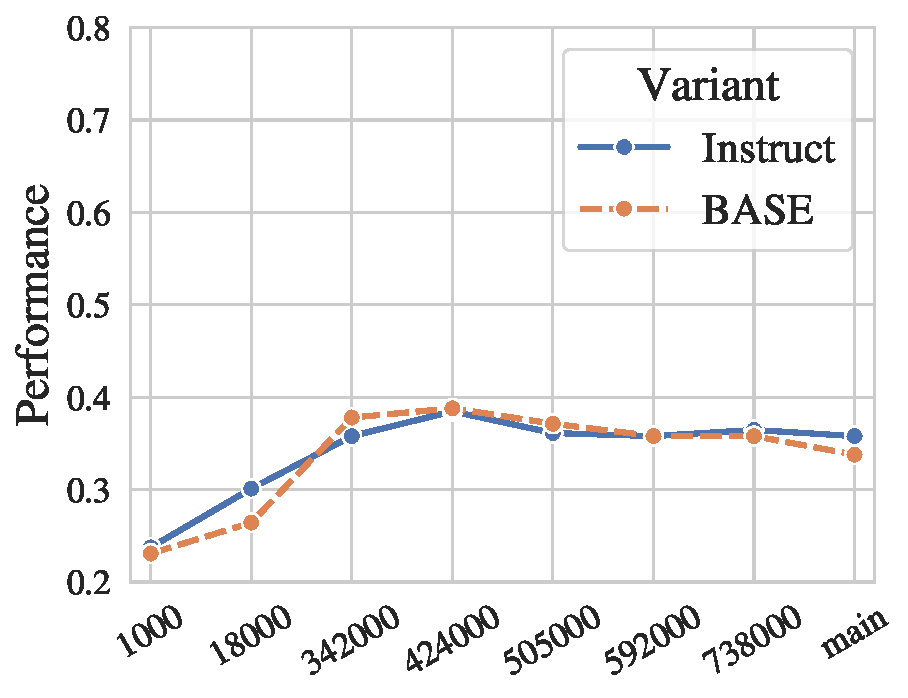
\includegraphics[width=\the\columnwidth]{figures/fig_files/it_ckpts/it_evalarc_challenge.pdf}
        \caption{ARC Challenge}
    \end{subfigure}%
    ~ 
    \begin{subfigure}[b]{0.3\textwidth}
    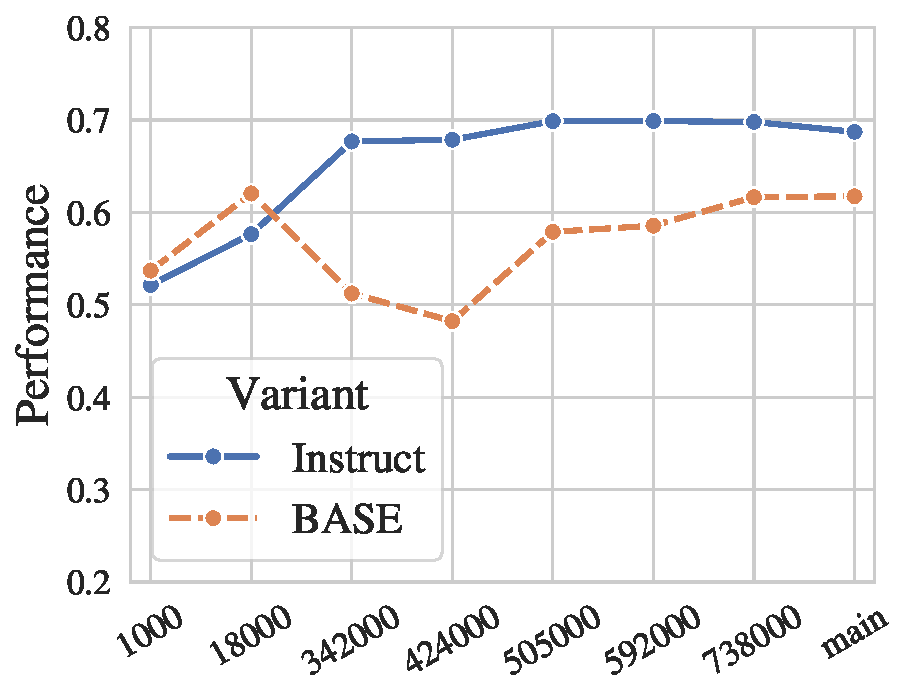
\includegraphics[width=\the\columnwidth]{figures/fig_files/it_ckpts/it_evalboolq.pdf}
        \caption{BoolQ}
    \end{subfigure}%
    \\
    \begin{subfigure}[b]{0.3\textwidth}
    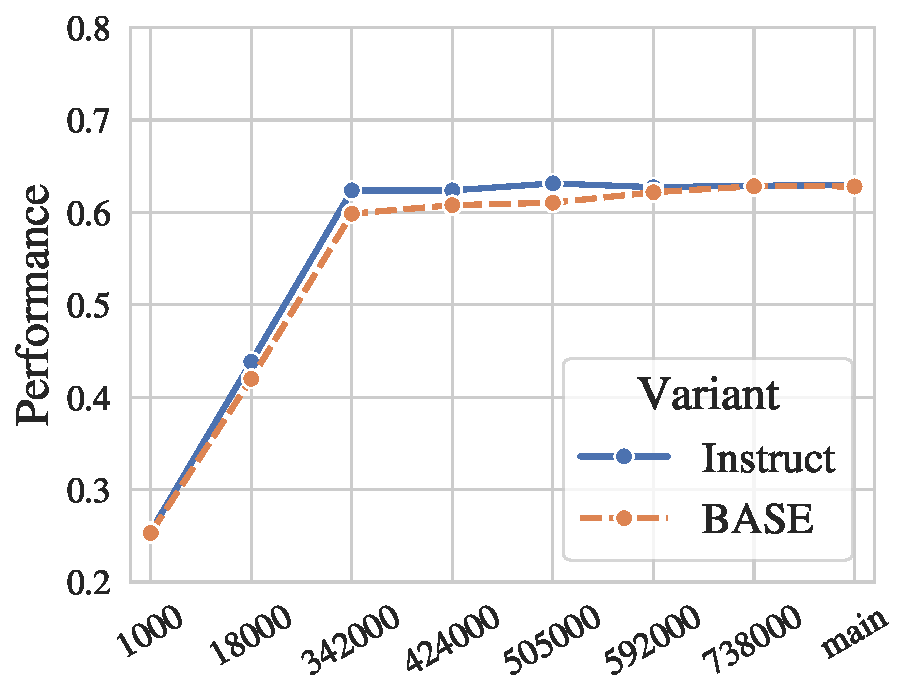
\includegraphics[width=\the\columnwidth]{figures/fig_files/it_ckpts/it_evalhellaswag.pdf}
        \caption{Hellaswag}
    \end{subfigure}%
    ~ 
    \begin{subfigure}[b]{0.3\textwidth}
    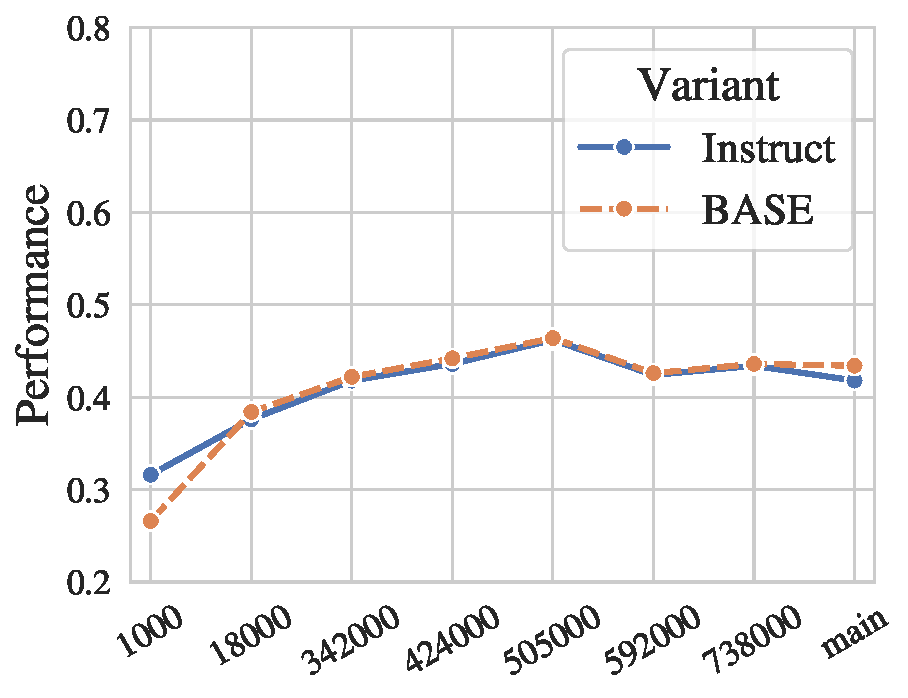
\includegraphics[width=\the\columnwidth]{figures/fig_files/it_ckpts/it_evalopenbookqa.pdf}
        \caption{Openbook QA}
    \end{subfigure}%
    ~ 
    \begin{subfigure}[b]{0.3\textwidth}
    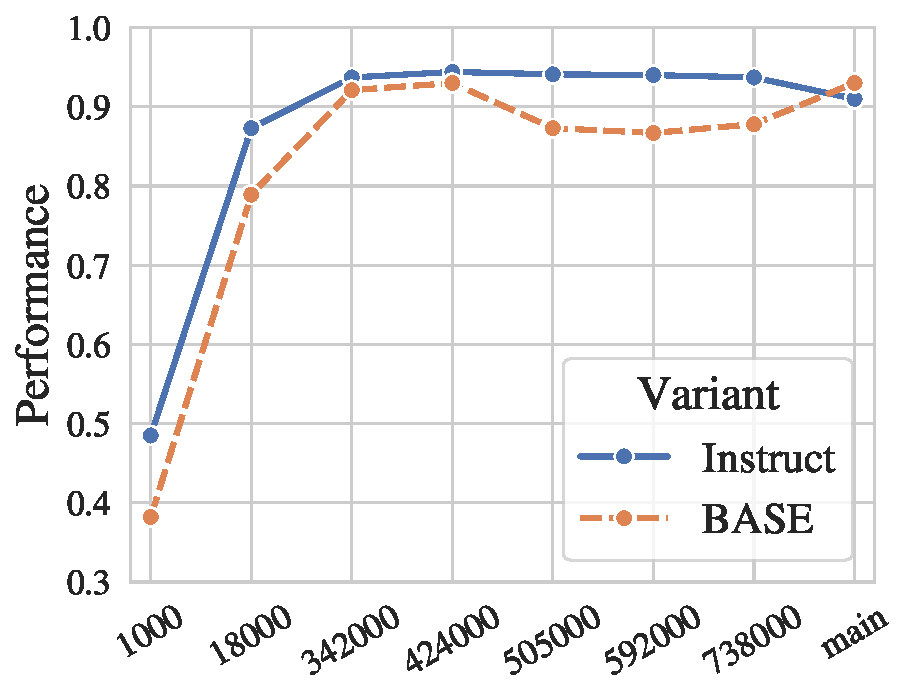
\includegraphics[width=\the\columnwidth]{figures/fig_files/it_ckpts/it_evalsciq.pdf}
        \caption{SciQ}
    \end{subfigure}%
    \caption{Model performance after instruction tuning on each pre-training step.}
    \label{fig:it-ckpt-perf}
\end{figure*}

\begin{figure*}[t!]
    \centering
    \begin{subfigure}[b]{0.3\textwidth}
    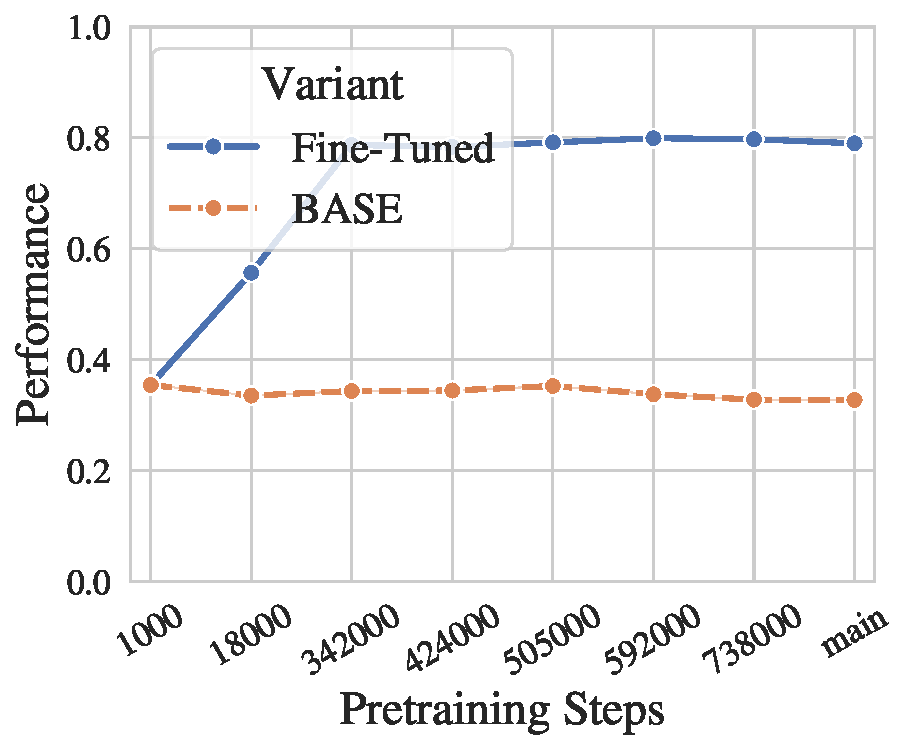
\includegraphics[width=\the\columnwidth]{figures/fig_files/ft_ckpts/sft_evalmnli_matched-trainmnli.pdf}
        \caption{MNLI matched}
    \end{subfigure}%
    ~ 
    \begin{subfigure}[b]{0.3\textwidth}
    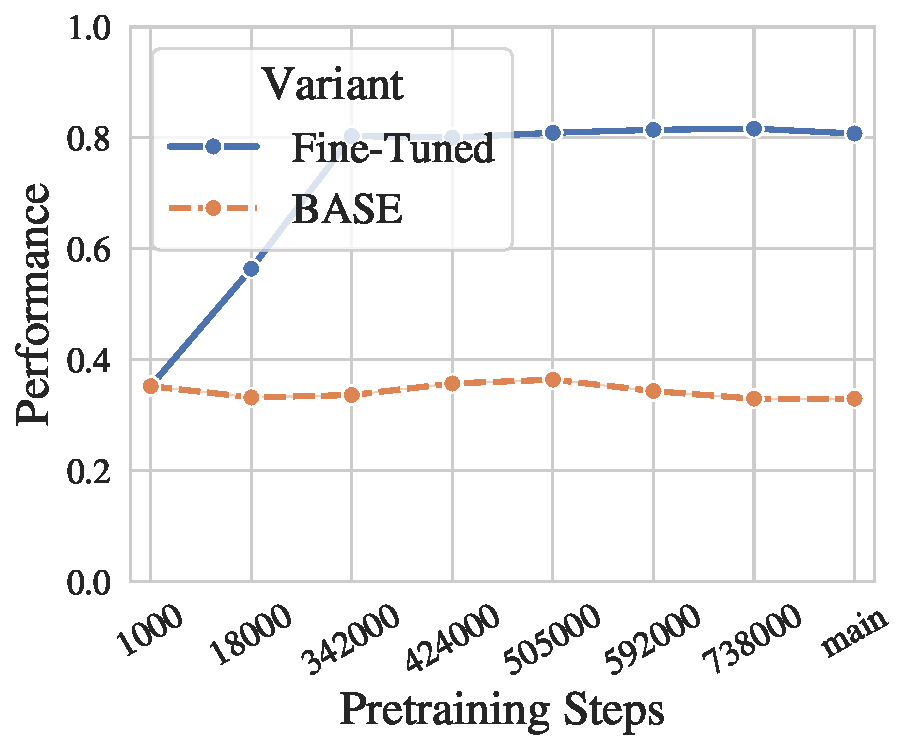
\includegraphics[width=\the\columnwidth]{figures/fig_files/ft_ckpts/sft_evalmnli_mismatched-trainmnli.pdf}
        \caption{MNLI mismatched}
    \end{subfigure}%
    ~ 
    \begin{subfigure}[b]{0.3\textwidth}
    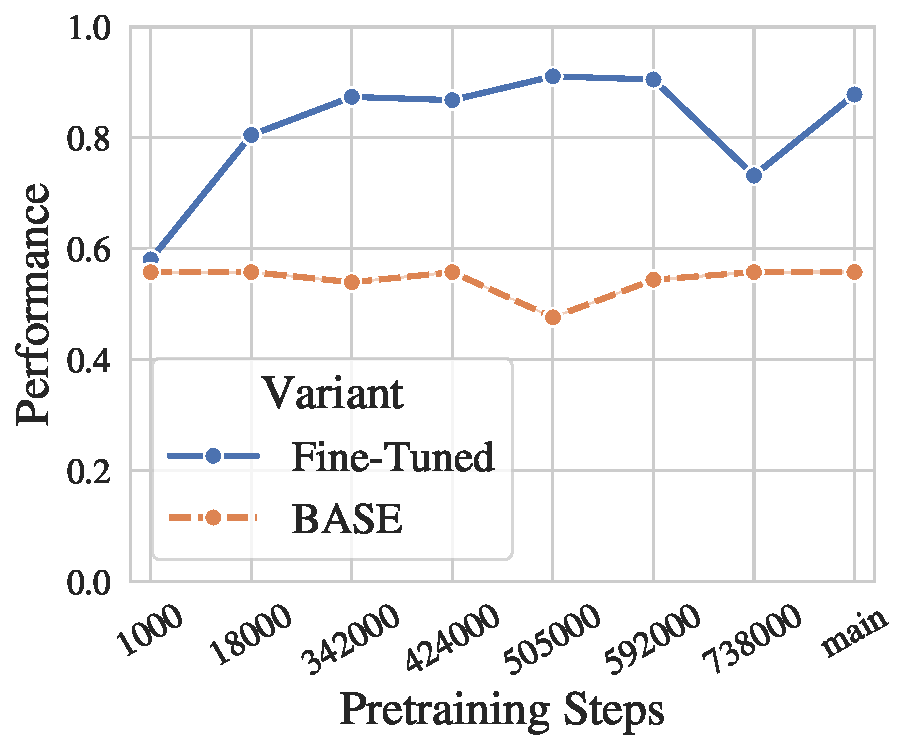
\includegraphics[width=\the\columnwidth]{figures/fig_files/ft_ckpts/sft_evalpaws-trainpaws.pdf}
        \caption{Paws}
    \end{subfigure}%
    \\
    \begin{subfigure}[b]{0.3\textwidth}
    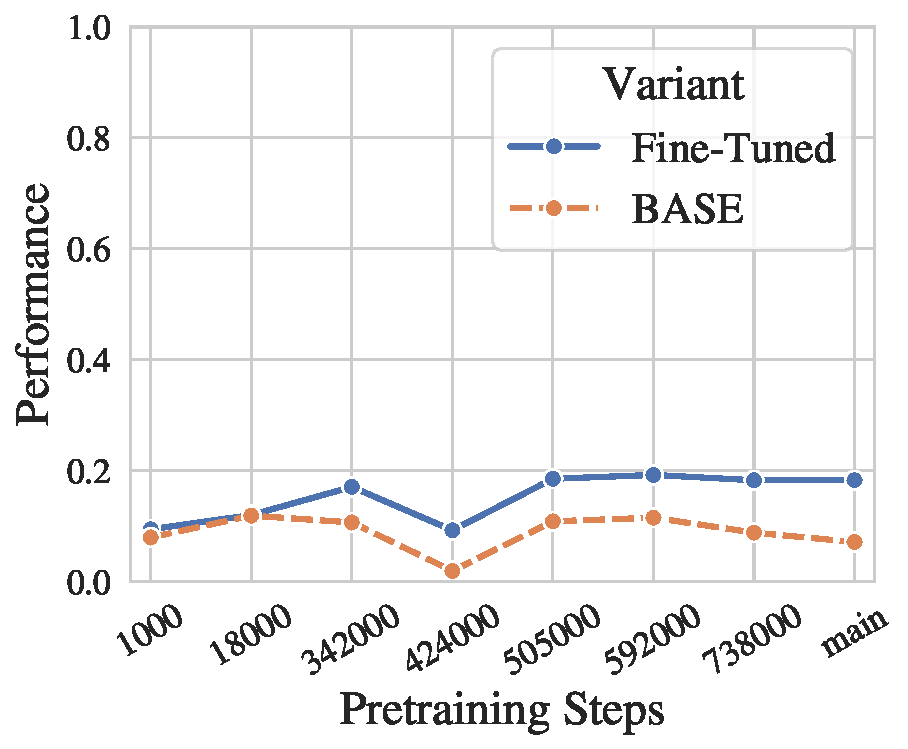
\includegraphics[width=\the\columnwidth]{figures/fig_files/ft_ckpts/sft_evalxsum-trainxsum.pdf}
        \caption{XSum}
    \end{subfigure}%
    ~ 
    \begin{subfigure}[b]{0.3\textwidth}
    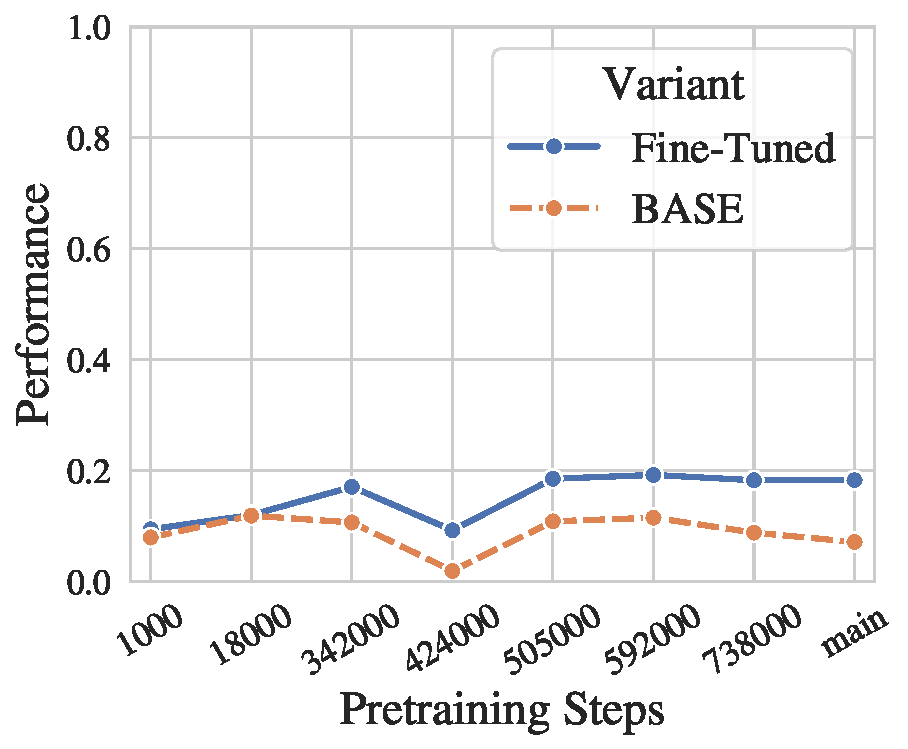
\includegraphics[width=\the\columnwidth]{figures/fig_files/ft_ckpts/sft_evalxsum-trainxsum.pdf}
        \caption{XLSum}
    \end{subfigure}%
    ~ 
    \begin{subfigure}[b]{0.3\textwidth}
    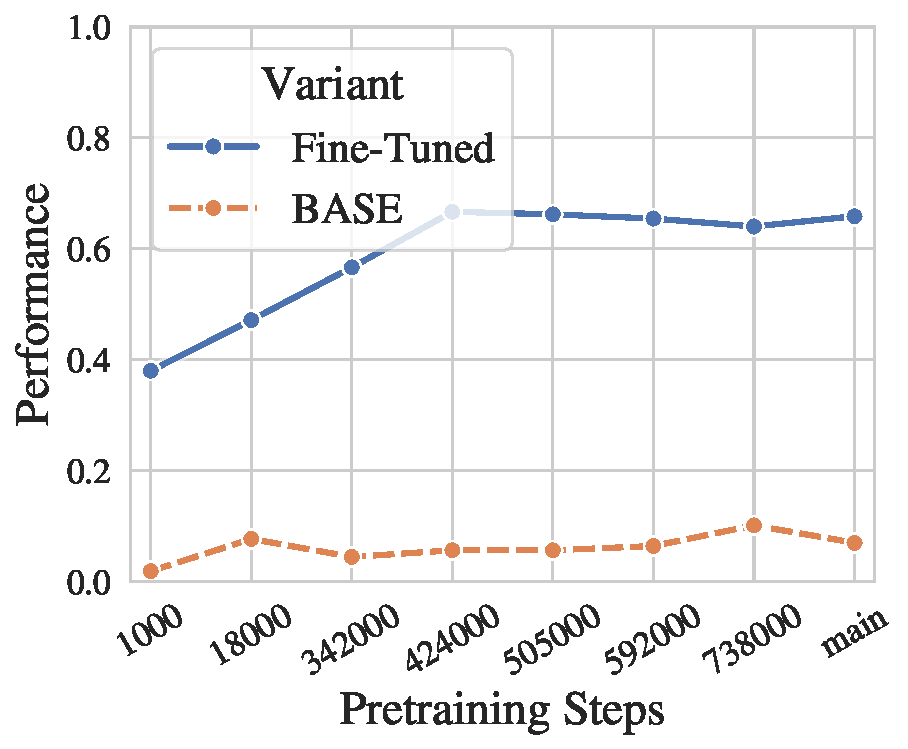
\includegraphics[width=\the\columnwidth]{figures/fig_files/ft_ckpts/sft_evalsocialiqa-trainsocialiqa.pdf}
        \caption{SocialIQA}
    \end{subfigure}%
    \caption{Model performance after supervised fine-tuning on each pre-training step.}
    \label{fig:sft-ckpt-perf}
\end{figure*}
We show the model performance on each dataset after supervised fine-tuning and instruction tuning correspondingly in Figure~\ref{fig:sft-ckpt-perf} and Figure~\ref{fig:it-ckpt-perf}.
The datasets that already show improvement during pre-training do not benefit from fine-tuning, while performance improve drastically on the datasets that the model has never learned during pre-training.

\paragraph{Out-of-domain Generalization}
The out-of-domain performance for each dataset with respect to pre-training steps is shown in Figure~\ref{fig:ood-sft-ckpt-perf}.
Overall, the model generalizes well after fine-tuning on NLI tasks, while its performance deteriorates when evaluated on out-of-domain paraphrase detection tasks.
\begin{figure*}[t!]
    \centering
    \begin{subfigure}[b]{0.25\textwidth}
    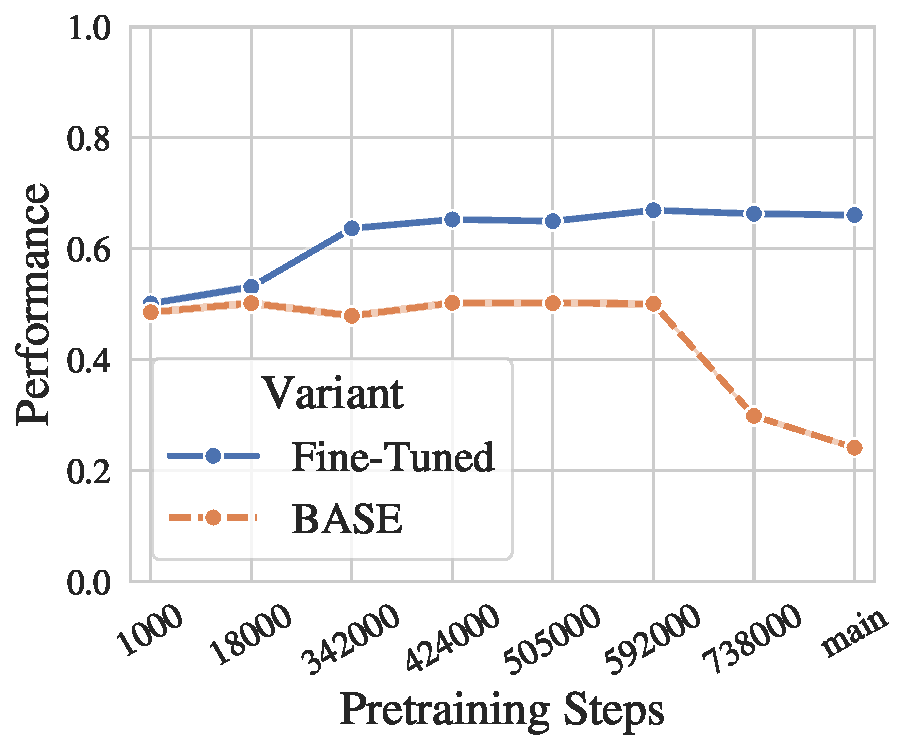
\includegraphics[width=\the\columnwidth]{figures/fig_files/ood/sft_evalrte-trainmnli.pdf}
        \caption{MNLI -> RTE}
    \end{subfigure}%
    ~ 
    \begin{subfigure}[b]{0.25\textwidth}
    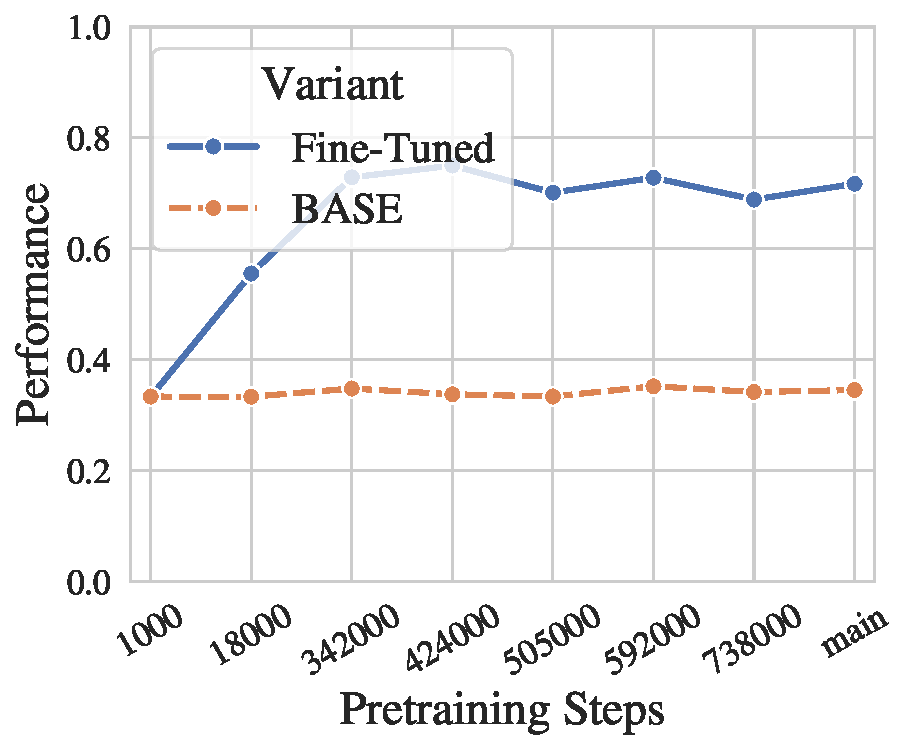
\includegraphics[width=\the\columnwidth]{figures/fig_files/ood/sft_evalgpt3nli-trainmnli.pdf}
        \caption{MNLI -> GPT3NLI}
    \end{subfigure}%
    ~ 
    \begin{subfigure}[b]{0.25\textwidth}
    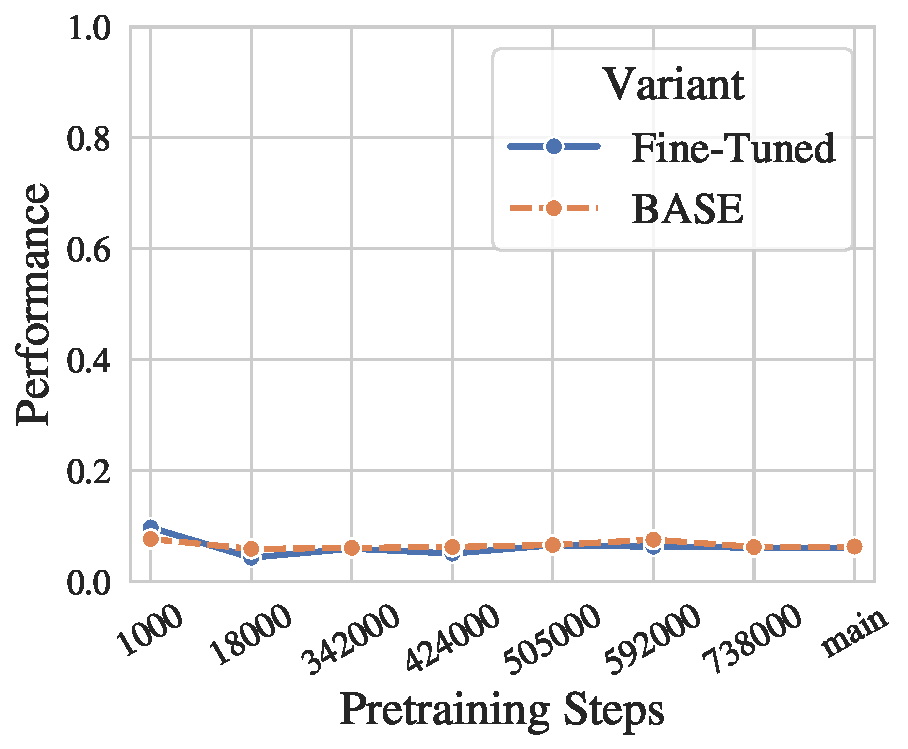
\includegraphics[width=\the\columnwidth]{figures/fig_files/ood/sft_evalcnn-trainxsum.pdf}
        \caption{XSum -> CNN}
    \end{subfigure}%
    \\
    \begin{subfigure}[b]{0.25\textwidth}
    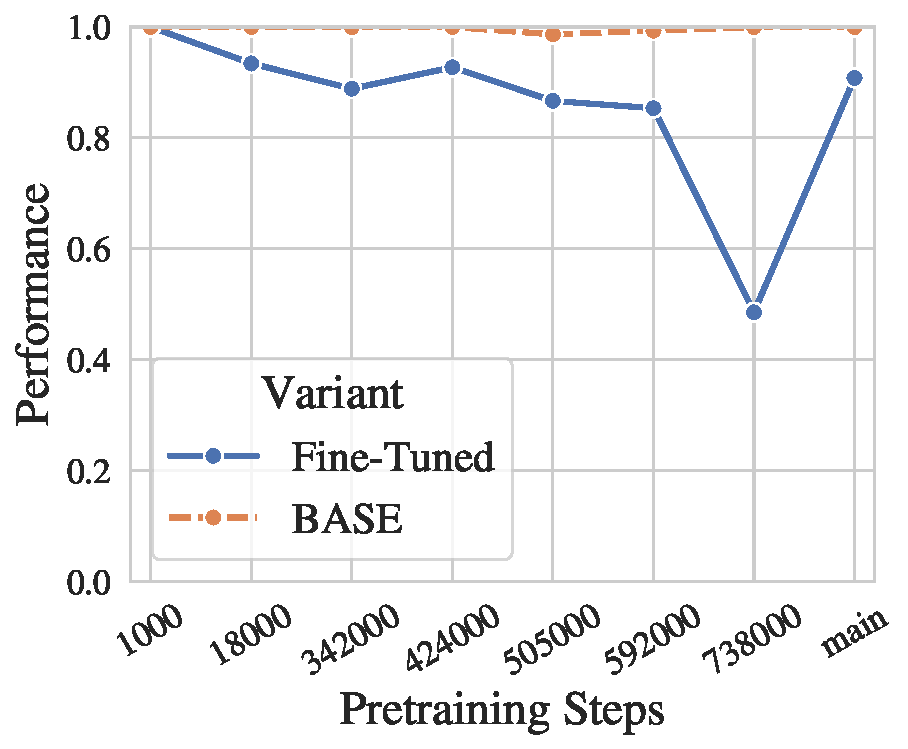
\includegraphics[width=\the\columnwidth]{figures/fig_files/ood/sft_evalqqp-trainpaws.pdf}
        \caption{Paws -> QQP}
    \end{subfigure}%
    ~ 
    \begin{subfigure}[b]{0.25\textwidth}
    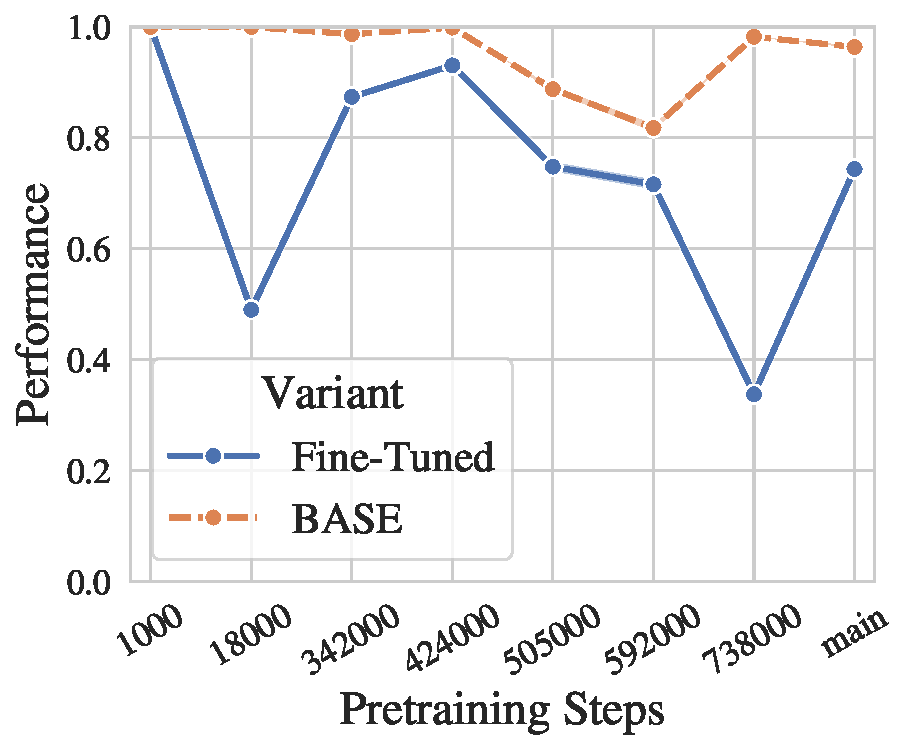
\includegraphics[width=\the\columnwidth]{figures/fig_files/ood/sft_evalstsb-trainpaws.pdf}
        \caption{Paws -> STS-B}
    \end{subfigure}%
    ~ 
    \begin{subfigure}[b]{0.25\textwidth}
    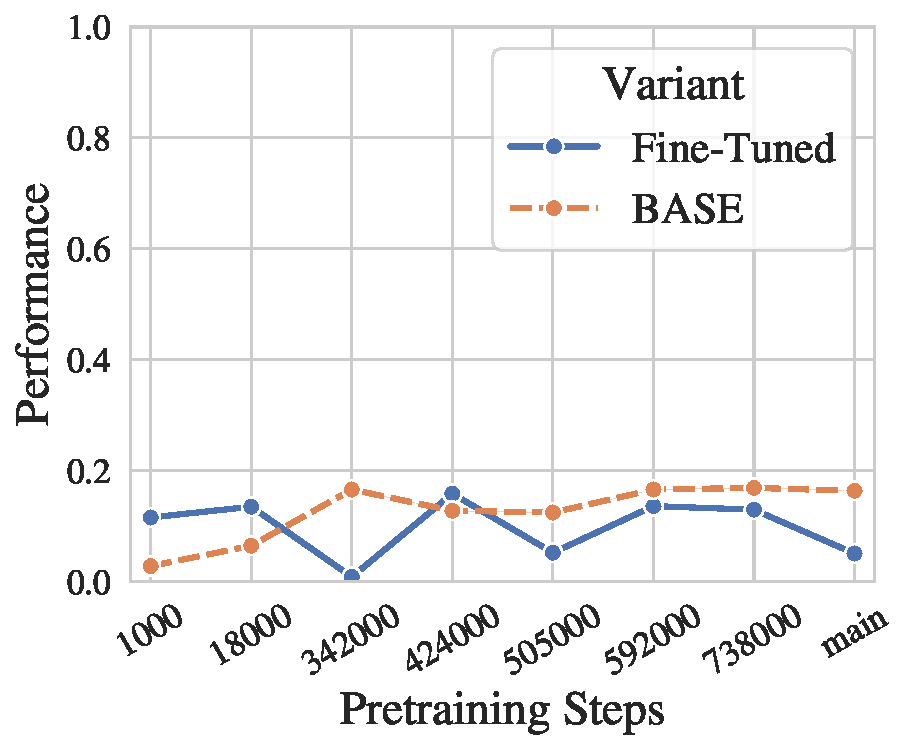
\includegraphics[width=\the\columnwidth]{figures/fig_files/ood/sft_evalsciq-trainsocialiqa.pdf}
        \caption{SocialIQA -> SciQ}
    \end{subfigure}%
    \begin{subfigure}[b]{0.25\textwidth}
    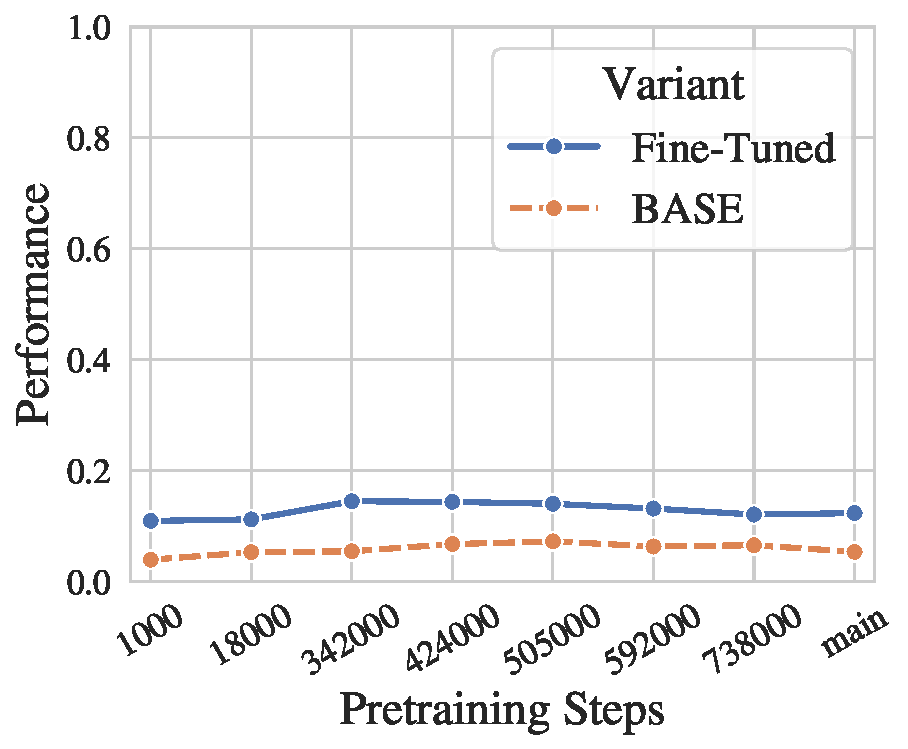
\includegraphics[width=\the\columnwidth]{figures/fig_files/ood/sft_evaltweetqa-trainsocialiqa.pdf}
        \caption{SocialIQA -> TweetQA}
    \end{subfigure}%
    \caption{Out-of-domain performance after supervised fine-tuning on each pre-training step.}
    \label{fig:ood-sft-ckpt-perf}
\end{figure*}

\paragraph{Cross-task Generalization}
The cross-task performance for each dataset with respect to pre-training steps is shown in Figure~\ref{fig:cross-task-ckpt-perf-class} and Figure~\ref{fig:cross-task-ckpt-perf-gen}.
\begin{figure*}[t!]
    \centering
    \begin{subfigure}[b]{0.3\textwidth}
    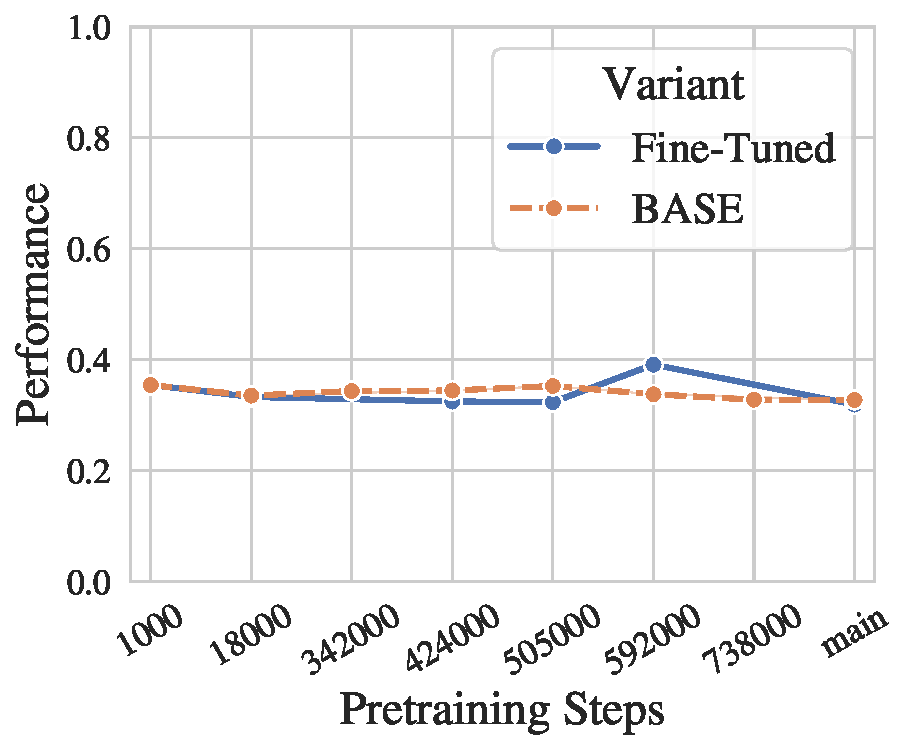
\includegraphics[width=\the\columnwidth]{figures/fig_files/cross-task/sft_evalmnli_matched-trainpaws.pdf}
        \caption{Paws -> MNLI}
    \end{subfigure}%
    ~ 
    \begin{subfigure}[b]{0.3\textwidth}
    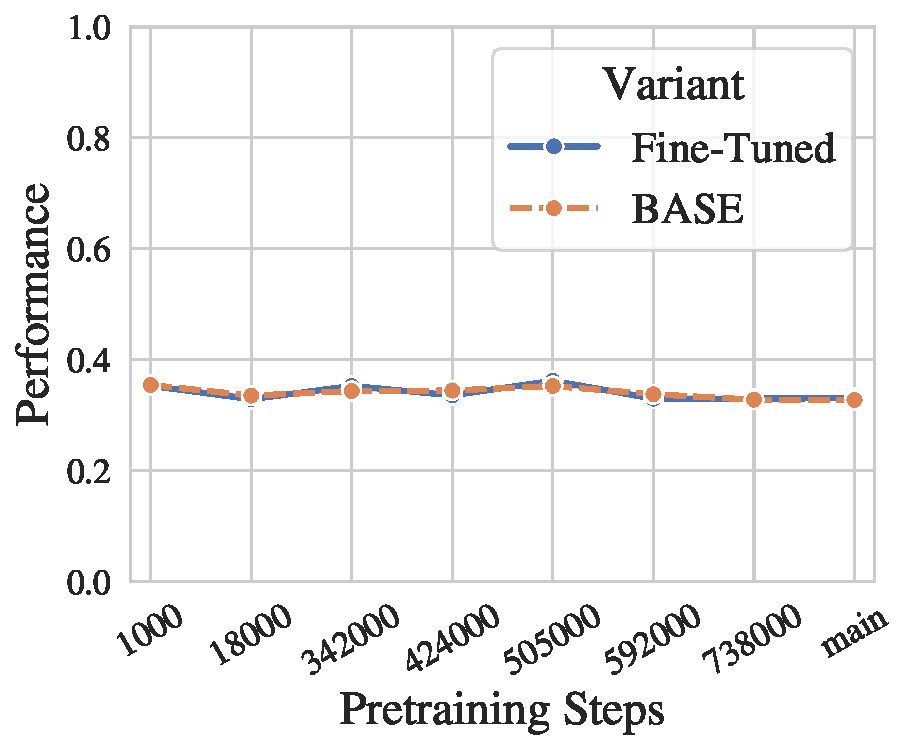
\includegraphics[width=\the\columnwidth]{figures/fig_files/cross-task/sft_evalmnli_matched-trainsocialiqa.pdf}
        \caption{SocialIQA -> MNLI}
    \end{subfigure}%
    ~ 
    \begin{subfigure}[b]{0.3\textwidth}
    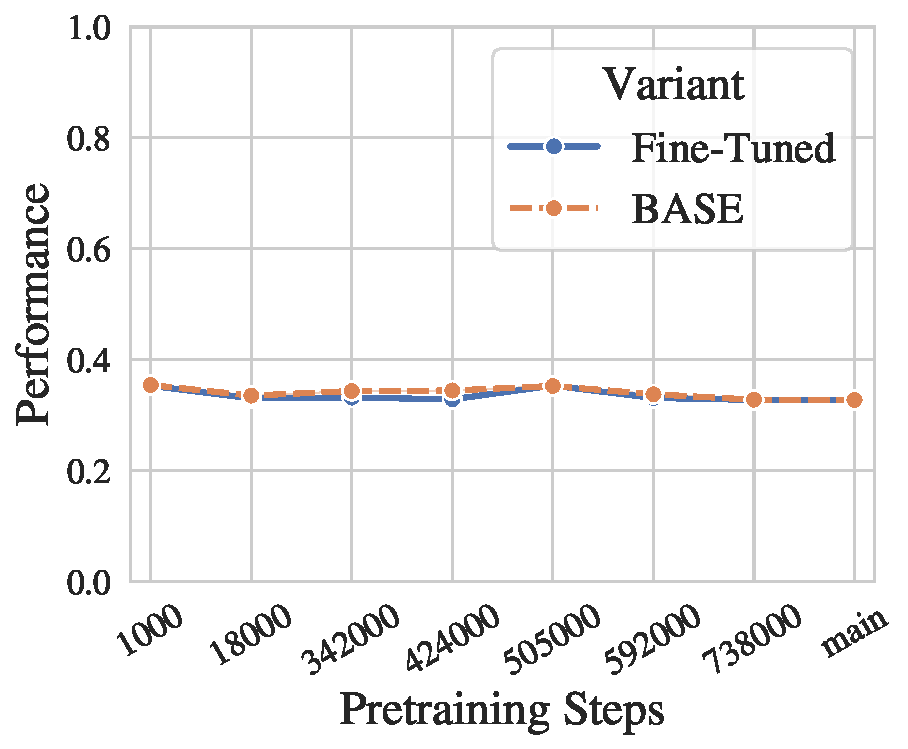
\includegraphics[width=\the\columnwidth]{figures/fig_files/cross-task/sft_evalmnli_matched-trainxsum.pdf}
        \caption{XSum -> MNLI}
    \end{subfigure}%
    \\
    \begin{subfigure}[b]{0.3\textwidth}
    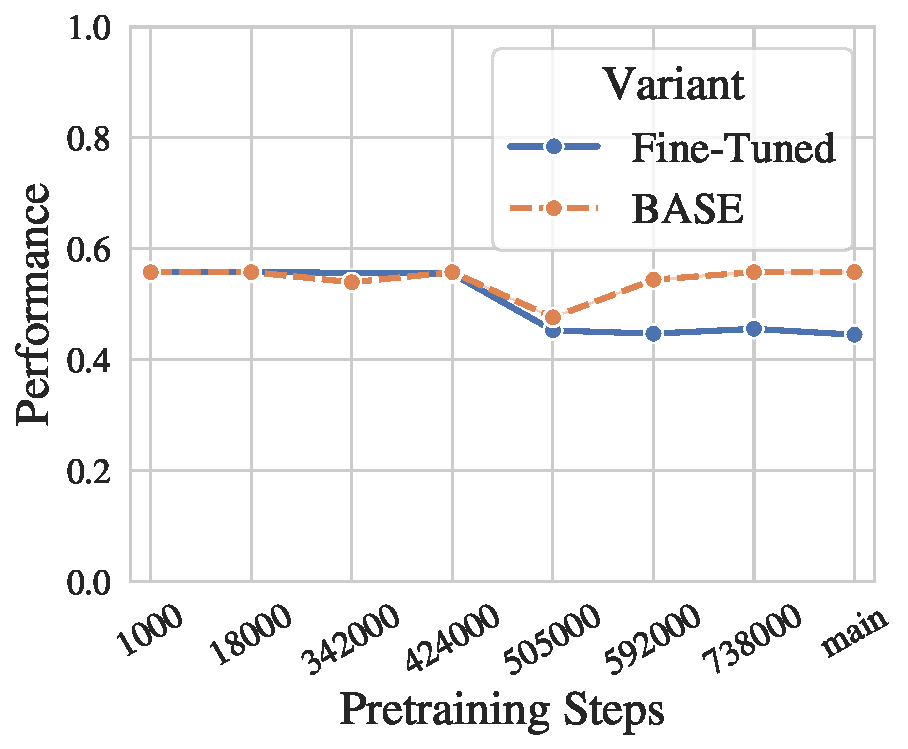
\includegraphics[width=\the\columnwidth]{figures/fig_files/cross-task/sft_evalpaws-trainmnli.pdf}
        \caption{MNLI -> Paws}
    \end{subfigure}%
    ~ 
    \begin{subfigure}[b]{0.3\textwidth}
    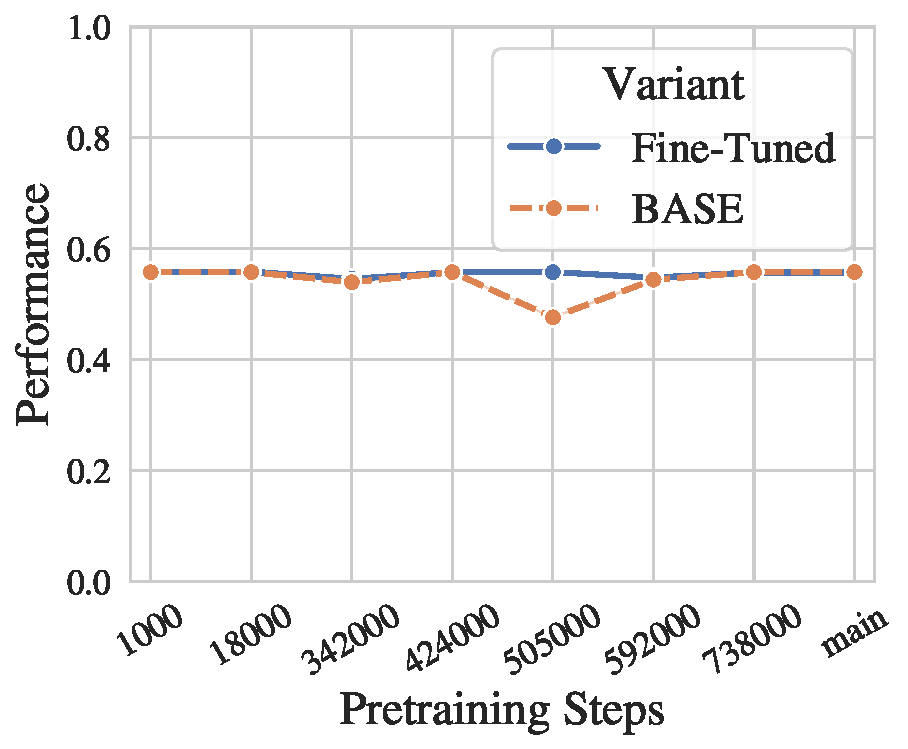
\includegraphics[width=\the\columnwidth]{figures/fig_files/cross-task/sft_evalpaws-trainsocialiqa.pdf}
        \caption{SocialIQA -> Paws}
    \end{subfigure}%
    ~ 
    \begin{subfigure}[b]{0.3\textwidth}
    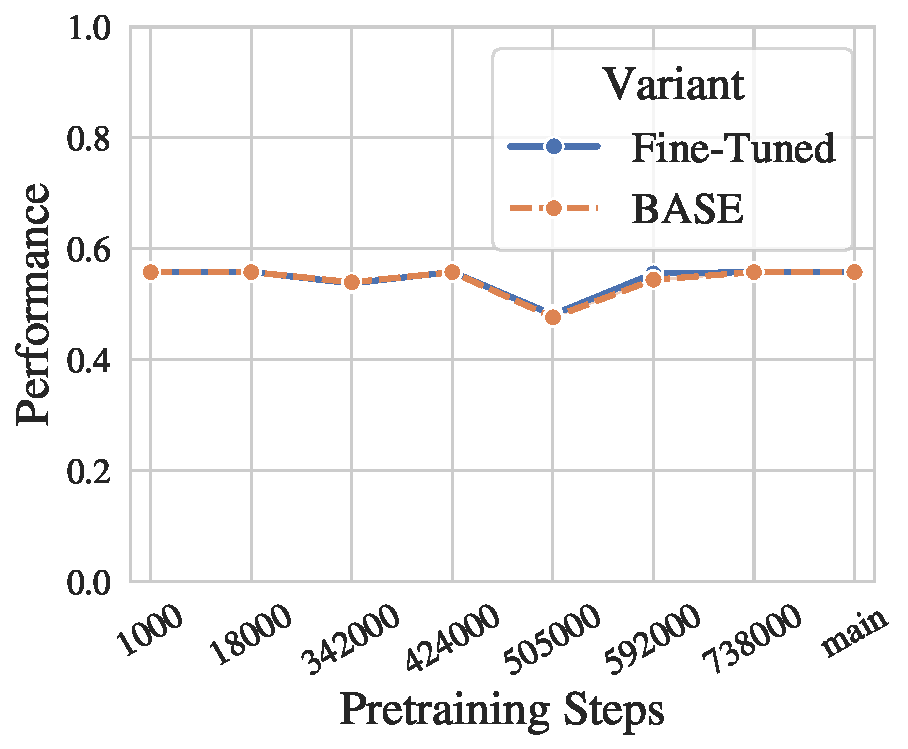
\includegraphics[width=\the\columnwidth]{figures/fig_files/cross-task/sft_evalpaws-trainxsum.pdf}
        \caption{XSum -> Paws}
    \end{subfigure}%
    \\
    \caption{Cross-task performance after supervised fine-tuning on each pre-training step. The model is fine-tuned on a classification task and evaluated on a generation task or a classification task with a different label set.}
    \label{fig:cross-task-ckpt-perf-class}
\end{figure*}

\begin{figure*}[t!]
    \centering
    \begin{subfigure}[b]{0.3\textwidth}
    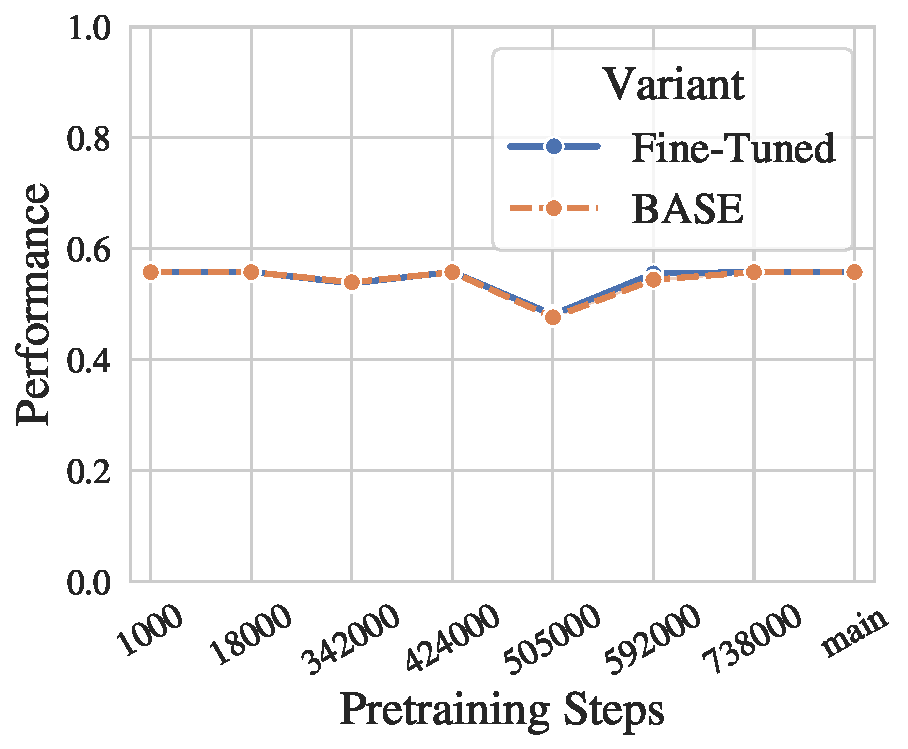
\includegraphics[width=\the\columnwidth]{figures/fig_files/cross-task/sft_evalpaws-trainxsum.pdf}
        \caption{Paws -> XSum}
    \end{subfigure}%
    ~ 
    \begin{subfigure}[b]{0.3\textwidth}
    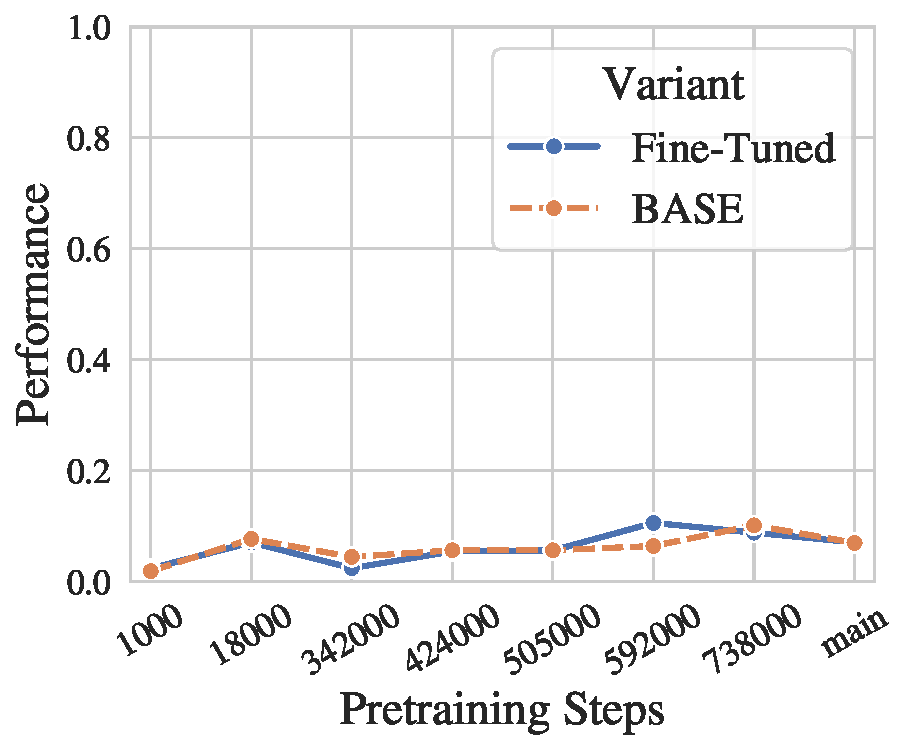
\includegraphics[width=\the\columnwidth]{figures/fig_files/cross-task/sft_evalsocialiqa-trainxsum.pdf}
        \caption{SocialIQA -> XSum}
    \end{subfigure}%
    ~ 
    \begin{subfigure}[b]{0.3\textwidth}
    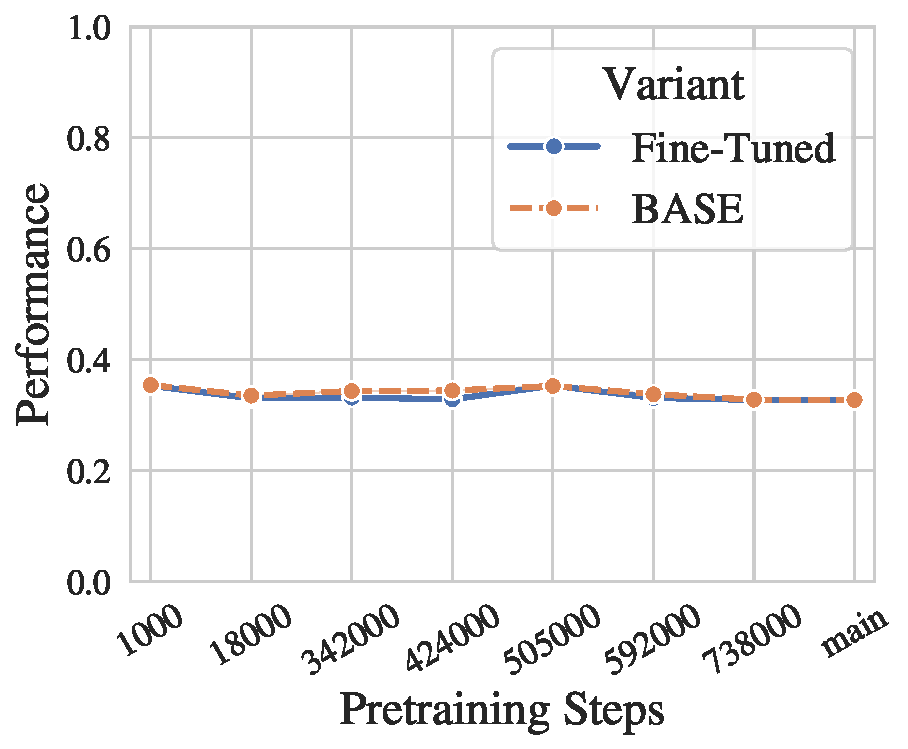
\includegraphics[width=\the\columnwidth]{figures/fig_files/cross-task/sft_evalmnli_matched-trainxsum.pdf}
        \caption{MNLI -> XSum}
    \end{subfigure}%
    \\
    \begin{subfigure}[b]{0.3\textwidth}
    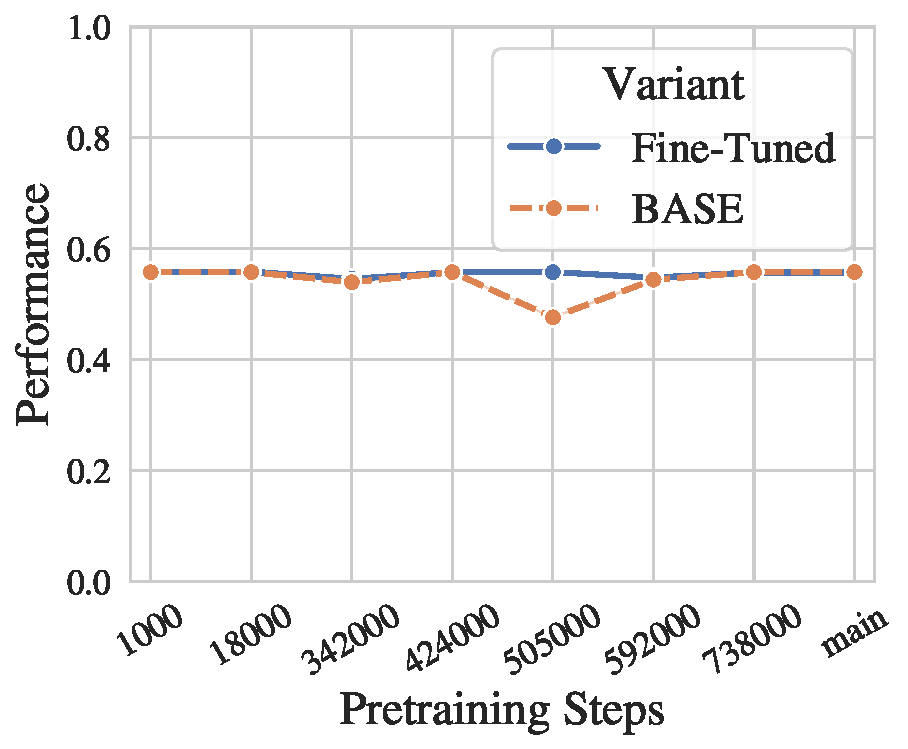
\includegraphics[width=\the\columnwidth]{figures/fig_files/cross-task/sft_evalpaws-trainsocialiqa.pdf}
        \caption{Paws -> SocialIQA}
    \end{subfigure}%
    ~ 
    \begin{subfigure}[b]{0.3\textwidth}
    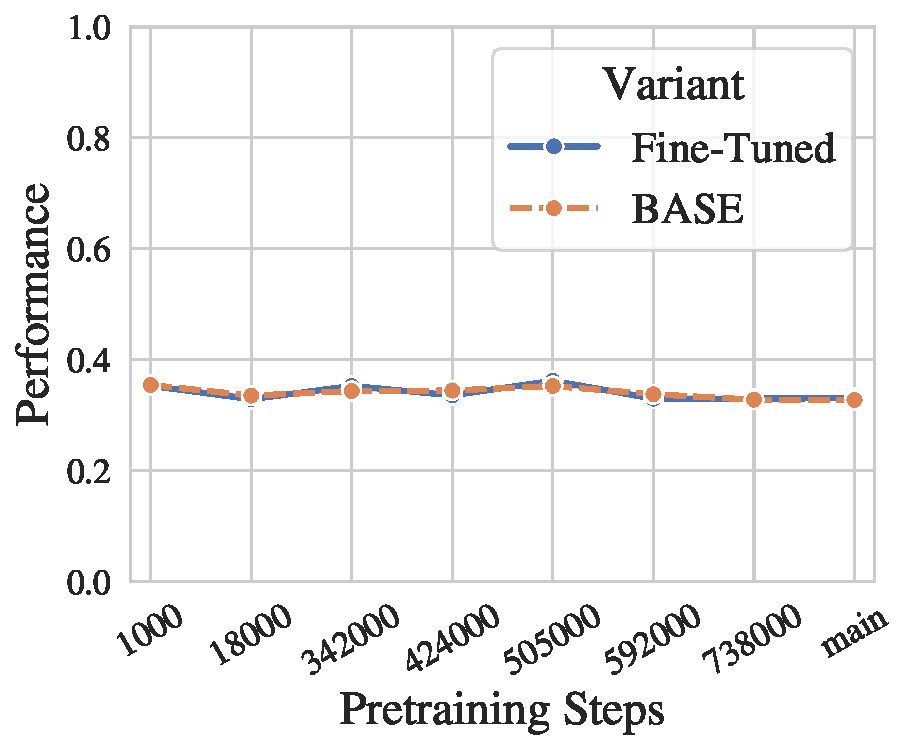
\includegraphics[width=\the\columnwidth]{figures/fig_files/cross-task/sft_evalmnli_matched-trainsocialiqa.pdf}
        \caption{MNLI -> SocialIQA}
    \end{subfigure}%
    ~ 
    \begin{subfigure}[b]{0.3\textwidth}
    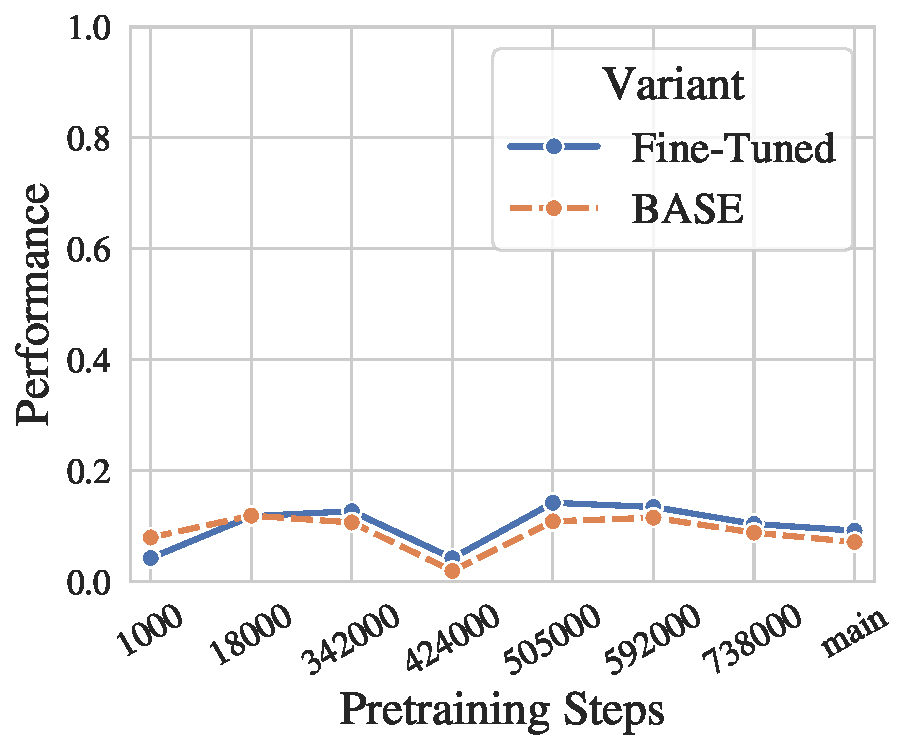
\includegraphics[width=\the\columnwidth]{figures/fig_files/cross-task/sft_evalxsum-trainsocialiqa.pdf}
        \caption{XSum -> SocialIQA}
    \end{subfigure}%
    \\
    \caption{Cross-task performance after supervised fine-tuning on each pre-training step. The model is fine-tuned on a generation task and evaluated on a classification task.}
    \label{fig:cross-task-ckpt-perf-gen}
\end{figure*}

\paragraph{Task-Format}
The performance of models on evaluation sets formatted with different prompt formatting method is shown in Figure~\ref{fig:app:task_format}.

\begin{table*}[t]
\scriptsize
\centering
\begin{tabular}{@{}cllll@{}}
\toprule
\multicolumn{1}{l}{\textbf{Task}} & \textbf{Default Prompt} & \textbf{Instruction Prompt} & \textbf{IO Prompt} & \textbf{Expected Output} \\ \midrule
\textbf{\begin{tabular}[c]{@{}c@{}}Summary\\ Generation\end{tabular}} & \begin{tabular}[c]{@{}l@{}}\#\#\# Input: \{document\}\\ \#\#\# Summary:\end{tabular} & \begin{tabular}[c]{@{}l@{}}Please read the following text: \{document\}\\ Provide a summary:\end{tabular} & \{document\} & \{summary\} \\ 
\arrayrulecolor{black!30}\midrule
\textbf{\begin{tabular}[c]{@{}c@{}}Question\\ Generation\end{tabular}} & \begin{tabular}[c]{@{}l@{}}\#\#\# Input: \{context\} \\ \#\#\# Answer: \{answer\}\\ \#\#\# Question:\end{tabular} & \begin{tabular}[c]{@{}l@{}}Given the context: \{context\}\\ And the answer: \{answer\}\\ Generate a suitable question:\end{tabular} & \begin{tabular}[c]{@{}l@{}}\{context\}\\ \{answer\}\end{tabular} & \{question\} \\ 
\arrayrulecolor{black!30}\midrule
\textbf{\begin{tabular}[c]{@{}c@{}}Natural Language\\ Inference\end{tabular}} & \begin{tabular}[c]{@{}l@{}}\#\#\# Input\_1: \{premise\} \\ \#\#\# Input\_2: \{hypothesis\}\\ \#\#\# Inference:\end{tabular} & \begin{tabular}[c]{@{}l@{}}Consider the following texts: Text 1: \{premise\} \\ Text 2: \{hypothesis\} The relation is\end{tabular} & \begin{tabular}[c]{@{}l@{}}\{premise\}\\ \{hypothesis\}\end{tabular} & \{label\} \\
\arrayrulecolor{black!30}\midrule
\textbf{Paraphrase Detection} & \begin{tabular}[c]{@{}l@{}}\#\#\# Input\_1: \{sentence1\} \\ \#\#\# Input\_2: \{sentence2\}\\ \#\#\# Paraphrase Classification:\end{tabular} & \begin{tabular}[c]{@{}l@{}}Let’s compare the two sentences: \\ Sentence\_1: \{sentence1\}\\ Sentence\_2: \{sentence2\} Are they paraphrasing?:\end{tabular} & \begin{tabular}[c]{@{}l@{}}\{sentence1\}\\ \{sentence2\}\end{tabular} & \{label\} \\ \arrayrulecolor{black}\bottomrule
\end{tabular}
\caption{Formatting of the prompts}
\label{tab:app:promptformat}
\end{table*}


\begin{figure*}[t!]
    \centering
    \begin{subfigure}[b]{0.4\textwidth}
    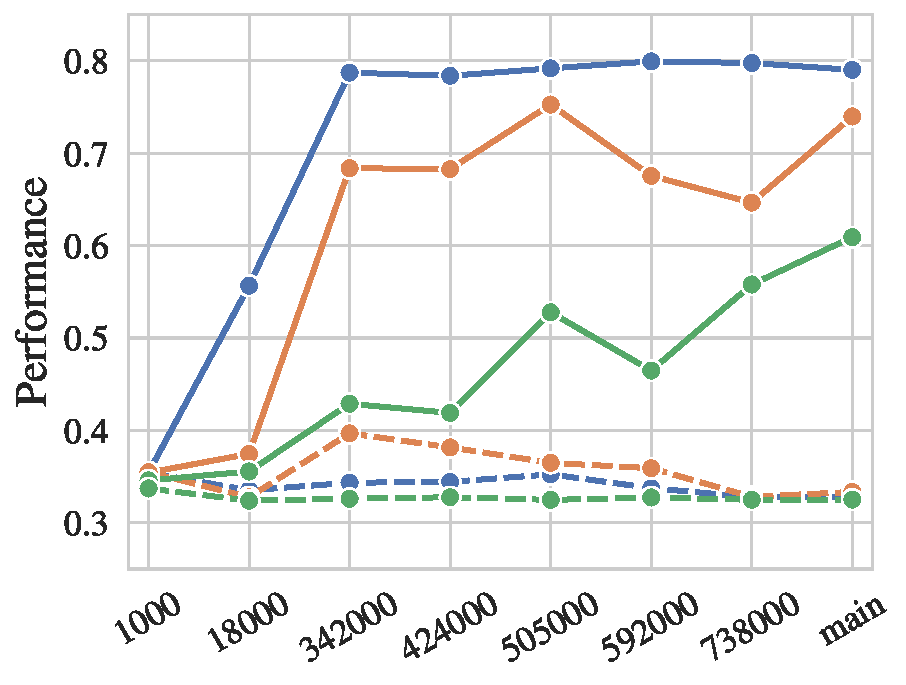
\includegraphics[width=\the\columnwidth]{figures/fig_files/task_format/task_format_evalmnli_matched-trainmnli.pdf}
        \caption{MNLI matched}
    \end{subfigure}%
    ~ 
    \begin{subfigure}[b]{0.4\textwidth}
    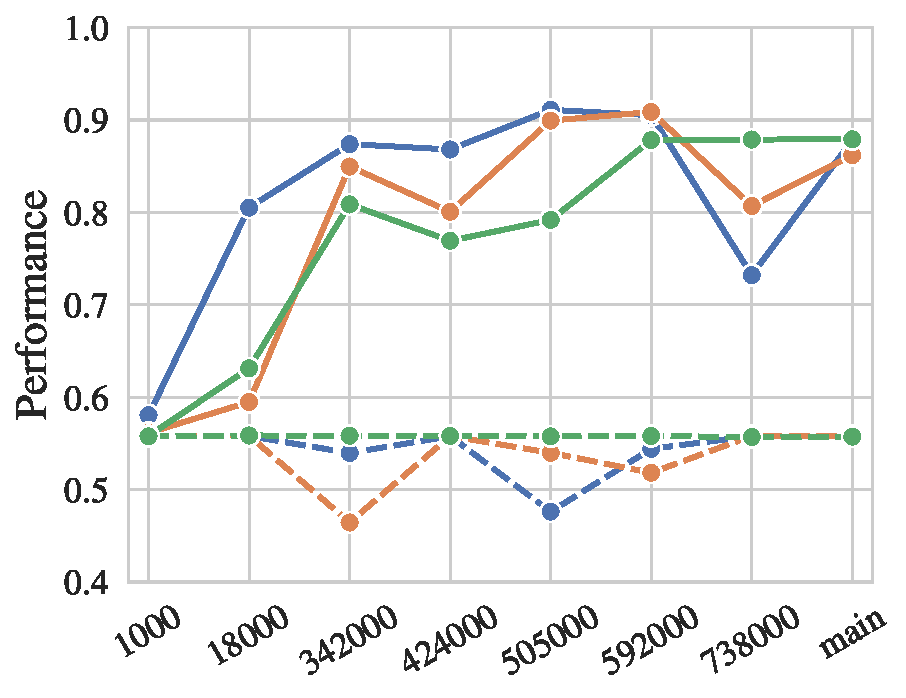
\includegraphics[width=\the\columnwidth]{figures/fig_files/task_format/task_format_evalpaws-trainpaws.pdf}
        \caption{Paws}
    \end{subfigure}%
    \\
    \begin{subfigure}[b]{0.4\textwidth}
    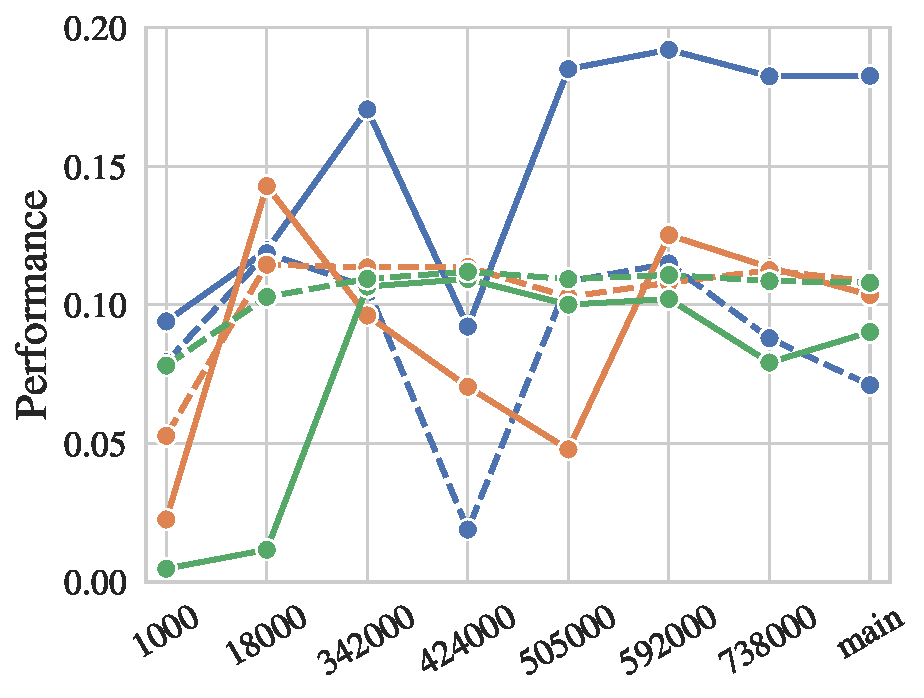
\includegraphics[width=\the\columnwidth]{figures/fig_files/task_format/task_format_evalxsum-trainxsum.pdf}
        \caption{XSum}
    \end{subfigure}%
    ~ 
    \begin{subfigure}[b]{0.55\textwidth}
    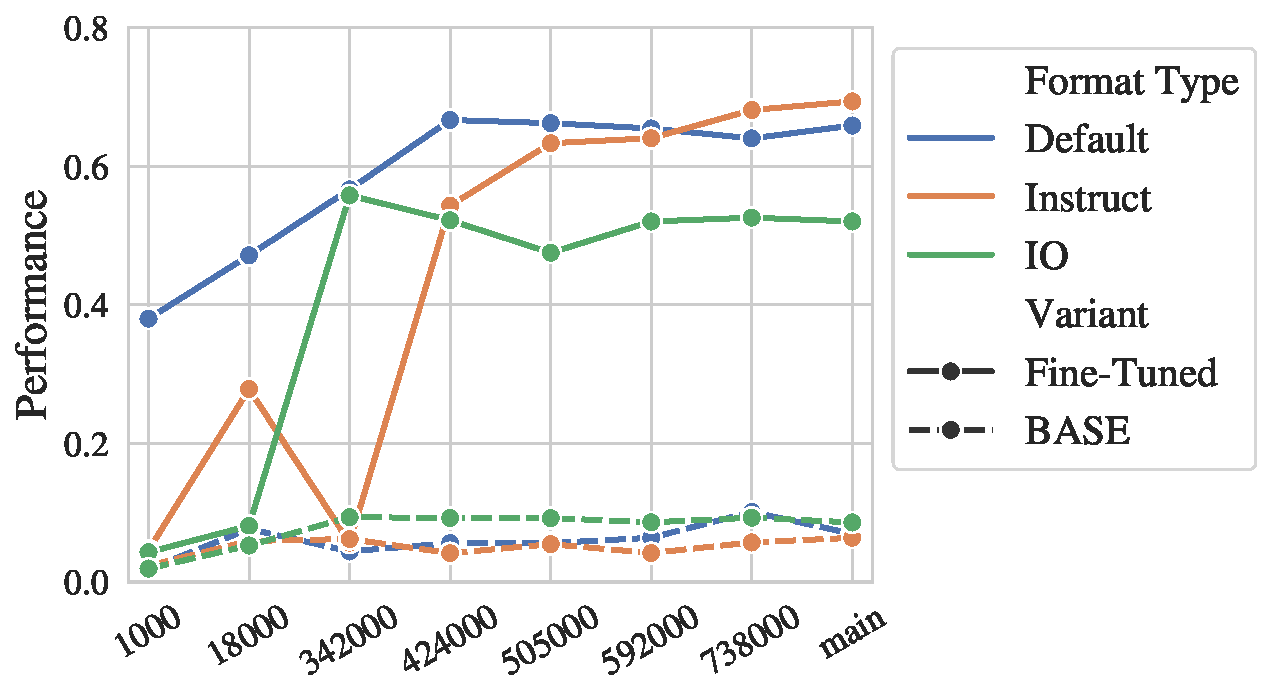
\includegraphics[width=\the\columnwidth]{figures/fig_files/task_format/task_format_evalsocialiqa-trainsocialiqa.pdf}
        \caption{SocialIQa}
    \end{subfigure}%

    \caption {Model performance with different task formats. }
  \label{fig:app:task_format}
\end{figure*}

\section{License of Artifacts}
We include the license of artifacts used in this paper in Table~\ref{app:tab:artifact}
\begin{table*}[t]
\scriptsize
\centering
\begin{tabular}{ccc|cc}
\toprule
\textbf{Name} & \textbf{License} &  & \textbf{Name} & \textbf{License} \\ \midrule
OLMo-1b & Apache 2.0 &  & SocialIQa & CC-BY \\
TULU & ODC-BY &  & \text{  }CNN/DailyMail & Apache 2.0 \\
ARC & CC BY-SA &  & TweetQA & CC BY-SA-4.0 \\
OpenbookQA & Apache 2.0 &  & MNLI & CC-BY-3.0 \\
Hellaswag & MIT &  & GPT3NLI & MIT \\
BoolQ & Apache 2.0 &  & RTE & N/A \\
SciQ & CC-BY-NC-3.0 &  & Paws & Free \\
XSum & MIT &  & QQP & Non-Commercial \\
XLSum & CC-BY-NC-SA 4.0 \text{  } &  & STS-B & Other \\ \bottomrule
\end{tabular}
\caption{License of artifacts used in this paper.}
\label{app:tab:artifact}
\end{table*}

\section{Performance Difference Numbers}
\label{sec:app:performance-numbers}
\begin{table}[t]
\centering
\small
\begin{tabular}{@{}rrr@{}}
\toprule
\multicolumn{1}{l}{\textbf{Checkpoint }} & \multicolumn{1}{c}{\begin{tabular}[c]{@{}c@{}}\textbf{  Learned in  } \\ \textbf{  Pre-train  }\end{tabular}} & \multicolumn{1}{c}{\begin{tabular}[c]{@{}c@{}}\textbf{  Learned in  } \\ \textbf{  Fine-Tune  }\end{tabular}} \\ \midrule
1000 & 0.048 & 0.062 \\
18000 & 0.048 & 0.149 \\
342000 & 0.004 & 0.286 \\
424000 & 0.01 & 0.297 \\
505000 & 0.03 & 0.304 \\
592000 & 0.027 & 0.297 \\
738000 & 0.021 & 0.264 \\
main & -0.005 & 0.290 \\ \bottomrule
\end{tabular}
\caption{Average performance change before and after fine-tuning for each checkpoint (Perf(Fine-tuned) - Perf(BASE)). The group that is never learned during pre-training is picked up by the model during fine-tuning.}
\label{tab:gain-tab-by-step}
\end{table}
The average performance change before and after fine-tuning for each checkpoint is shown in Table~\ref{tab:gain-tab-by-step}.
The data in this table is used to create Figure~\ref{fig:finding:ptftcompare}.

\section{Full Performance Table}
Due to availability of space and the amount of fine-tuned checkpoints, we omit displaying all exact metric values in the paper.
The performance of each fine-tuned variant on each dataset can be found in the \texttt{csv} file in the code base.


\section{Generalization Taxonomy}
\label{sec:app:generalization-taxo}
Following the generalization taxonomy in \citealp{hupkes2023taxonomy}, the evaluation card is included in Table~\ref{app:tab:gen_eval_card}.

\newcommand{\tabularwidth}{\textwidth}

\newcommand{\expone}{$\square$}
\newcommand{\exptwo}{$\bigtriangleup$}
        
\renewcommand{\arraystretch}{1.1}         
\setlength{\tabcolsep}{0mm}         
\begin{tabular}{|p{\tabularwidth}<{\centering}|}         
\hline
               
\rowcolor{gray!60}               
\textbf{Motivation} \\               
\footnotesize
\begin{tabular}{p{0.25\tabularwidth}<{\centering} p{0.25\tabularwidth}<{\centering} p{0.25\tabularwidth}<{\centering} p{0.25\tabularwidth}<{\centering}}                        
\textit{Practical} & \textit{Cognitive} & \textit{Intrinsic} & \textit{Fairness}\\
\expone\hspace{0.8mm}\exptwo\hspace{0.8mm}		%
& 		%
& 		%
& 		%

\vspace{2mm} \\
\end{tabular}\\
               
\rowcolor{gray!60}               
\textbf{Generalisation type} \\               
\footnotesize
\begin{tabular}{m{0.21\tabularwidth}<{\centering} m{0.2\tabularwidth}<{\centering} m{0.13\tabularwidth}<{\centering} m{0.13\tabularwidth}<{\centering} m{0.13\tabularwidth}<{\centering} m{0.2\tabularwidth}<{\centering}}                   
\textit{Compositional} & \textit{Structural} & \textit{Cross Task} & \textit{Cross Language} & \textit{Cross Domain} & \textit{Robustness}\\
& 		%
& \exptwo\hspace{0.8mm}		%
& 		%
& \expone\hspace{0.8mm}		%
& 		%

\vspace{2mm} \\
\end{tabular}\\
             
\rowcolor{gray!60}             
\textbf{Shift type} \\             
\footnotesize
\begin{tabular}{p{0.25\tabularwidth}<{\centering} p{0.25\tabularwidth}<{\centering} p{0.25\tabularwidth}<{\centering} p{0.25\tabularwidth}<{\centering}}                        
\textit{Covariate} & \textit{Label} & \textit{Full} & \textit{Assumed}\\  
\expone\hspace{0.8mm}		%
& \exptwo\hspace{0.8mm}		%
& 		%
& 		%

\vspace{2mm} \\
\end{tabular}\\
             
\rowcolor{gray!60}             
\textbf{Shift source} \\             
\footnotesize
\begin{tabular}{p{0.25\tabularwidth}<{\centering} p{0.25\tabularwidth}<{\centering} p{0.25\tabularwidth}<{\centering} p{0.25\tabularwidth}<{\centering}}                          
\textit{Naturally occuring} & \textit{Partitioned natural} & \textit{Generated shift} & \textit{Fully generated}\\
\expone\hspace{0.8mm}\exptwo\hspace{0.8mm}		%
& 		%
& 		%
& 		%

\vspace{2mm} \\
\end{tabular}\\
             
\rowcolor{gray!60}             
\textbf{Shift locus}\\             
\footnotesize
\begin{tabular}{p{0.25\tabularwidth}<{\centering} p{0.25\tabularwidth}<{\centering} p{0.25\tabularwidth}<{\centering} p{0.25\tabularwidth}<{\centering}}                         
\textit{Train--test} & \textit{Finetune train--test} & \textit{Pretrain--train} & \textit{Pretrain--test}\\
& \expone\hspace{0.8mm}\exptwo\hspace{0.8mm}		%
& 		%
& 		%

\vspace{2mm} \\
\end{tabular}\\
\hline
\end{tabular}
\label{app:tab:gen_eval_card}